\documentclass[tikz,border=10pt]{standalone}
\usepackage{tikz}
\begin{document}

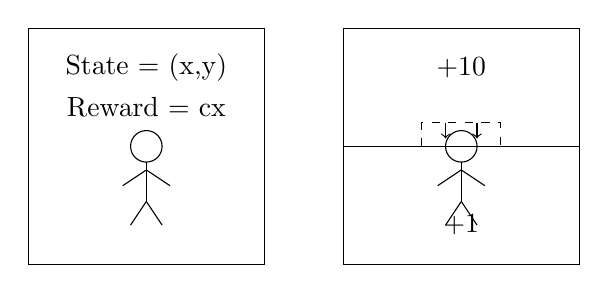
\begin{tikzpicture}
    % Left box
    \draw (0,0) rectangle (3,3);
    \node at (1.5,2.5) {State = (x,y)};
    \node at (1.5,2) {Reward = cx};
    % Stick figure in the left box
    \draw (1.5,1.5) circle (0.2); % head
    \draw (1.5,1.3) -- (1.5,0.8); % body
    \draw (1.5,1.2) -- (1.2,1); % left arm
    \draw (1.5,1.2) -- (1.8,1); % right arm
    \draw (1.5,0.8) -- (1.3,0.5); % left leg
    \draw (1.5,0.8) -- (1.7,0.5); % right leg

    % Right box
    \draw (4,0) rectangle (7,3);
    \draw (4,1.5) -- (7,1.5); % horizontal line
    \node at (5.5,2.5) {+10};
    \node at (5.5,0.5) {+1};
    % Stick figure in the right box
    \draw (5.5,1.5) circle (0.2); % head
    \draw (5.5,1.3) -- (5.5,0.8); % body
    \draw (5.5,1.2) -- (5.2,1); % left arm
    \draw (5.5,1.2) -- (5.8,1); % right arm
    \draw (5.5,0.8) -- (5.3,0.5); % left leg
    \draw (5.5,0.8) -- (5.7,0.5); % right leg

    % Treadmill arrows
    \draw[dashed] (5,1.5) rectangle (6,1.8);
    \draw[->] (5.3,1.8) -- (5.3,1.6);
    \draw[->] (5.7,1.8) -- (5.7,1.6);

\end{tikzpicture}

\end{document}